\documentclass[14pt]{extbook}
\usepackage{multicol, enumerate, enumitem, hyperref, color, soul, setspace, parskip, fancyhdr} %General Packages
\usepackage{amssymb, amsthm, amsmath, bbm, latexsym, units, mathtools} %Math Packages
\everymath{\displaystyle} %All math in Display Style
% Packages with additional options
\usepackage[headsep=0.5cm,headheight=12pt, left=1 in,right= 1 in,top= 1 in,bottom= 1 in]{geometry}
\usepackage[usenames,dvipsnames]{xcolor}
\usepackage{dashrule}  % Package to use the command below to create lines between items
\newcommand{\litem}[1]{\item#1\hspace*{-1cm}\rule{\textwidth}{0.4pt}}
\pagestyle{fancy}
\lhead{Progress Quiz 8}
\chead{}
\rhead{Version C}
\lfoot{4553-3922}
\cfoot{}
\rfoot{Fall 2020}
\begin{document}

\begin{enumerate}
\litem{
Solve the quadratic equation below. Then, choose the intervals that the solutions $x_1$ and $x_2$ belong to, with $x_1 \leq x_2$.\[ 25x^{2} +60 x + 36 = 0 \]\begin{enumerate}[label=\Alph*.]
\item \( x_1 \in [-4.5, -2.48] \text{ and } x_2 \in [-0.52, -0.28] \)
\item \( x_1 \in [-1.51, -0.92] \text{ and } x_2 \in [-1.29, -1.11] \)
\item \( x_1 \in [-30.82, -29.54] \text{ and } x_2 \in [-30.12, -29.96] \)
\item \( x_1 \in [-2.57, -2.22] \text{ and } x_2 \in [-0.62, -0.54] \)
\item \( x_1 \in [-6.23, -5.1] \text{ and } x_2 \in [-0.25, -0.23] \)

\end{enumerate} }
\litem{
Solve the quadratic equation below. Then, choose the intervals that the solutions $x_1$ and $x_2$ belong to, with $x_1 \leq x_2$.\[ 25x^{2} -60 x + 36 = 0 \]\begin{enumerate}[label=\Alph*.]
\item \( x_1 \in [0.16, 0.39] \text{ and } x_2 \in [5.7, 6.06] \)
\item \( x_1 \in [0.37, 0.42] \text{ and } x_2 \in [2.83, 3.98] \)
\item \( x_1 \in [29.98, 30.17] \text{ and } x_2 \in [29.54, 30.08] \)
\item \( x_1 \in [0.46, 0.71] \text{ and } x_2 \in [2.32, 2.91] \)
\item \( x_1 \in [1.15, 1.21] \text{ and } x_2 \in [1.09, 1.42] \)

\end{enumerate} }
\litem{
Factor the quadratic below. Then, choose the intervals that contain the constants in the form $(ax+b)(cx+d); b \leq d.$\[ 24x^{2} +38 x + 15 \]\begin{enumerate}[label=\Alph*.]
\item \( a \in [-0.05, 1.94], \hspace*{5mm} b \in [17, 21], \hspace*{5mm} c \in [-0.32, 1.14], \text{ and } \hspace*{5mm} d \in [20, 22] \)
\item \( a \in [1.24, 3.56], \hspace*{5mm} b \in [-1, 7], \hspace*{5mm} c \in [11.09, 13.53], \text{ and } \hspace*{5mm} d \in [3, 9] \)
\item \( a \in [11.37, 12.92], \hspace*{5mm} b \in [-1, 7], \hspace*{5mm} c \in [1.12, 2.39], \text{ and } \hspace*{5mm} d \in [3, 9] \)
\item \( a \in [3.73, 4.76], \hspace*{5mm} b \in [-1, 7], \hspace*{5mm} c \in [4.91, 6.12], \text{ and } \hspace*{5mm} d \in [3, 9] \)
\item \( \text{None of the above.} \)

\end{enumerate} }
\litem{
Graph the equation below.\[ f(x) = (x-1)^2 + 19 \]\begin{enumerate}[label=\Alph*.]
\begin{multicols}{2}\item 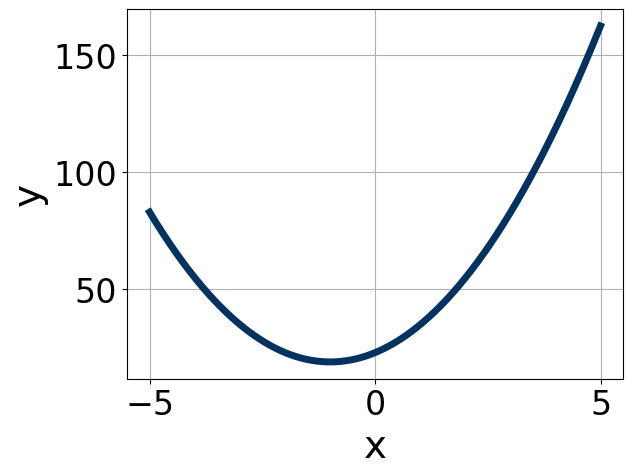
\includegraphics[width = 0.3\textwidth]{../Figures/quadraticEquationToGraphCopyAC.png}\item 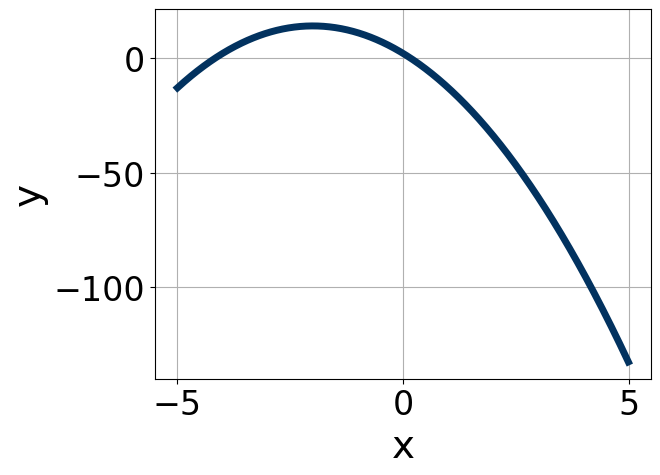
\includegraphics[width = 0.3\textwidth]{../Figures/quadraticEquationToGraphCopyBC.png}\item 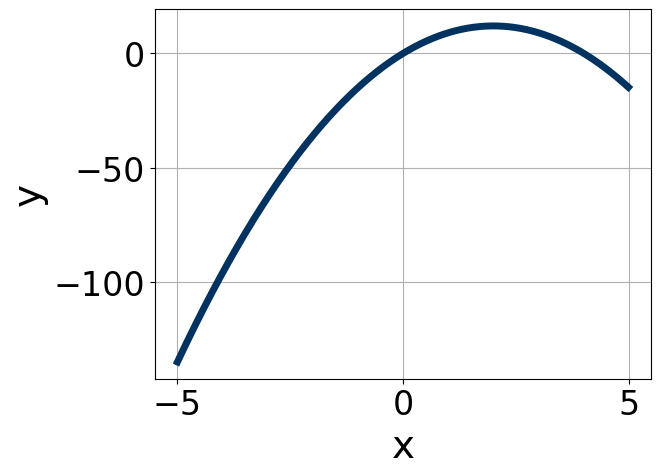
\includegraphics[width = 0.3\textwidth]{../Figures/quadraticEquationToGraphCopyCC.png}\item 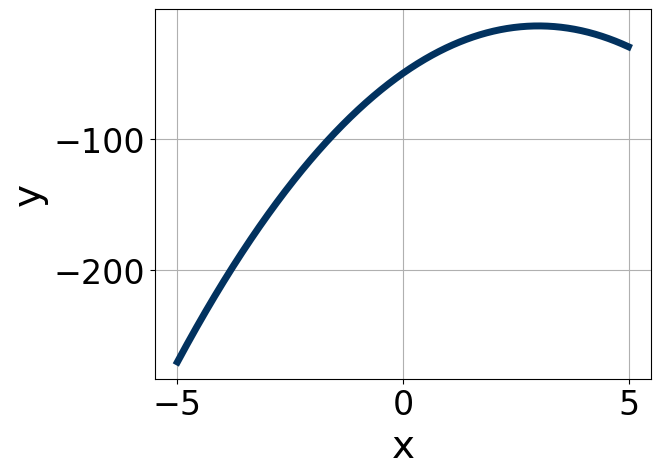
\includegraphics[width = 0.3\textwidth]{../Figures/quadraticEquationToGraphCopyDC.png}\end{multicols}\item None of the above.
\end{enumerate} }
\litem{
Solve the quadratic equation below. Then, choose the intervals that the solutions belong to, with $x_1 \leq x_2$ (if they exist).\[ -15x^{2} -8 x + 6 = 0 \]\begin{enumerate}[label=\Alph*.]
\item \( x_1 \in [-21.98, -20.74] \text{ and } x_2 \in [19.6, 21.2] \)
\item \( x_1 \in [-6.53, -6.22] \text{ and } x_2 \in [13, 15.5] \)
\item \( x_1 \in [-0.78, 0.53] \text{ and } x_2 \in [0.8, 2] \)
\item \( x_1 \in [-1.13, -0.47] \text{ and } x_2 \in [-0.3, 0.5] \)
\item \( \text{There are no Real solutions.} \)

\end{enumerate} }
\litem{
Solve the quadratic equation below. Then, choose the intervals that the solutions belong to, with $x_1 \leq x_2$ (if they exist).\[ -18x^{2} -7 x + 2 = 0 \]\begin{enumerate}[label=\Alph*.]
\item \( x_1 \in [-3.49, -2.91] \text{ and } x_2 \in [9.72, 10.59] \)
\item \( x_1 \in [-1, -0.57] \text{ and } x_2 \in [-0.83, 0.47] \)
\item \( x_1 \in [-14.87, -13.4] \text{ and } x_2 \in [13.23, 14.13] \)
\item \( x_1 \in [-0.33, 0.04] \text{ and } x_2 \in [0.48, 0.99] \)
\item \( \text{There are no Real solutions.} \)

\end{enumerate} }
\litem{
Write the equation of the graph presented below in the form $f(x)=ax^2+bx+c$, assuming  $a=1$ or $a=-1$. Then, choose the intervals that $a, b,$ and $c$ belong to.
\begin{center}
    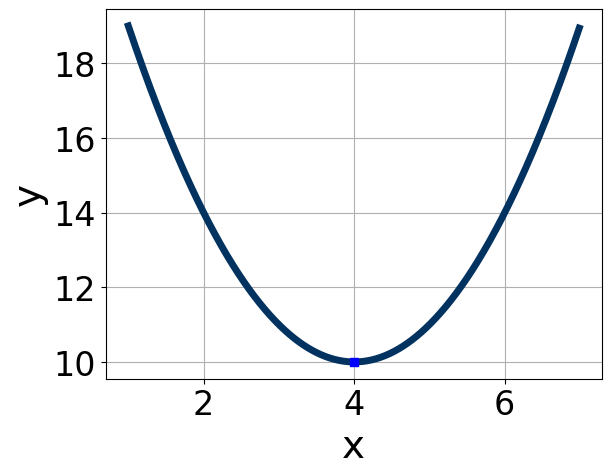
\includegraphics[width=0.5\textwidth]{../Figures/quadraticGraphToEquationC.png}
\end{center}
\begin{enumerate}[label=\Alph*.]
\item \( a \in [0.6, 2], \hspace*{5mm} b \in [8, 10], \text{ and } \hspace*{5mm} c \in [17.4, 19.1] \)
\item \( a \in [0.6, 2], \hspace*{5mm} b \in [-9, -1], \text{ and } \hspace*{5mm} c \in [17.4, 19.1] \)
\item \( a \in [-1.4, 0.4], \hspace*{5mm} b \in [8, 10], \text{ and } \hspace*{5mm} c \in [-14.7, -13.5] \)
\item \( a \in [0.6, 2], \hspace*{5mm} b \in [-9, -1], \text{ and } \hspace*{5mm} c \in [13.7, 16] \)
\item \( a \in [-1.4, 0.4], \hspace*{5mm} b \in [-9, -1], \text{ and } \hspace*{5mm} c \in [-14.7, -13.5] \)

\end{enumerate} }
\litem{
Factor the quadratic below. Then, choose the intervals that contain the constants in the form $(ax+b)(cx+d); b \leq d.$\[ 36x^{2} +60 x + 25 \]\begin{enumerate}[label=\Alph*.]
\item \( a \in [1.3, 4.1], \hspace*{5mm} b \in [2, 13], \hspace*{5mm} c \in [17.8, 19.4], \text{ and } \hspace*{5mm} d \in [3, 11] \)
\item \( a \in [3.4, 6.6], \hspace*{5mm} b \in [2, 13], \hspace*{5mm} c \in [4.4, 9.1], \text{ and } \hspace*{5mm} d \in [3, 11] \)
\item \( a \in [10.5, 12.4], \hspace*{5mm} b \in [2, 13], \hspace*{5mm} c \in [2, 5.6], \text{ and } \hspace*{5mm} d \in [3, 11] \)
\item \( a \in [-2, 1.3], \hspace*{5mm} b \in [26, 33], \hspace*{5mm} c \in [-1.6, 2.5], \text{ and } \hspace*{5mm} d \in [30, 34] \)
\item \( \text{None of the above.} \)

\end{enumerate} }
\litem{
Write the equation of the graph presented below in the form $f(x)=ax^2+bx+c$, assuming  $a=1$ or $a=-1$. Then, choose the intervals that $a, b,$ and $c$ belong to.
\begin{center}
    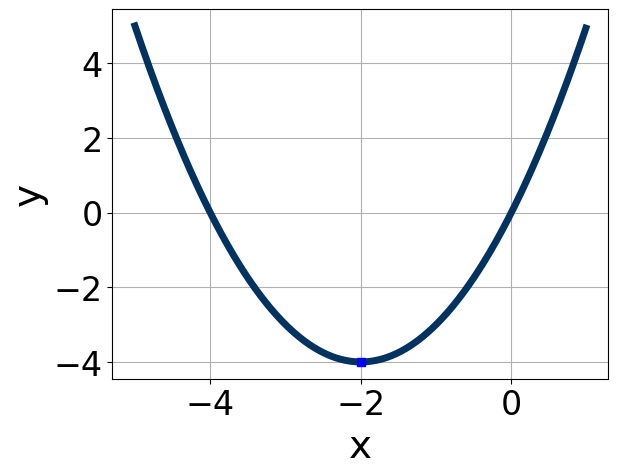
\includegraphics[width=0.5\textwidth]{../Figures/quadraticGraphToEquationCopyC.png}
\end{center}
\begin{enumerate}[label=\Alph*.]
\item \( a \in [0, 2], \hspace*{5mm} b \in [5, 12], \text{ and } \hspace*{5mm} c \in [22, 25] \)
\item \( a \in [-3, 0], \hspace*{5mm} b \in [-10, -4], \text{ and } \hspace*{5mm} c \in [-10, -5] \)
\item \( a \in [0, 2], \hspace*{5mm} b \in [-10, -4], \text{ and } \hspace*{5mm} c \in [22, 25] \)
\item \( a \in [-3, 0], \hspace*{5mm} b \in [5, 12], \text{ and } \hspace*{5mm} c \in [-24, -23] \)
\item \( a \in [-3, 0], \hspace*{5mm} b \in [5, 12], \text{ and } \hspace*{5mm} c \in [-10, -5] \)

\end{enumerate} }
\litem{
Graph the equation below.\[ f(x) = -(x-2)^2 - 13 \]\begin{enumerate}[label=\Alph*.]
\begin{multicols}{2}\item 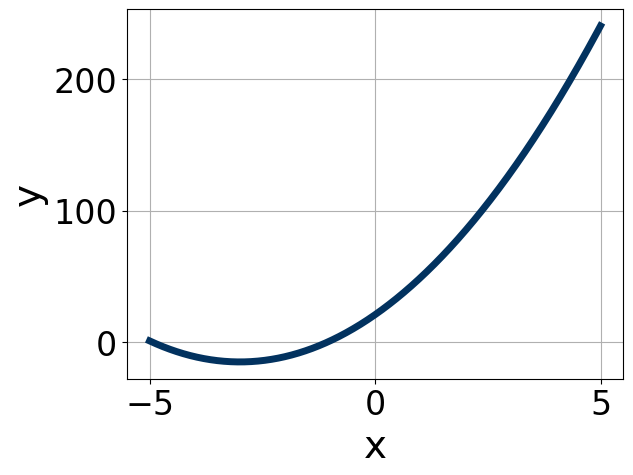
\includegraphics[width = 0.3\textwidth]{../Figures/quadraticEquationToGraphAC.png}\item 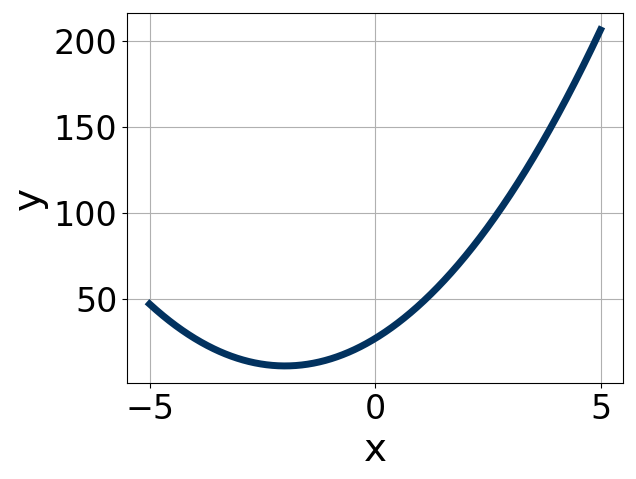
\includegraphics[width = 0.3\textwidth]{../Figures/quadraticEquationToGraphBC.png}\item 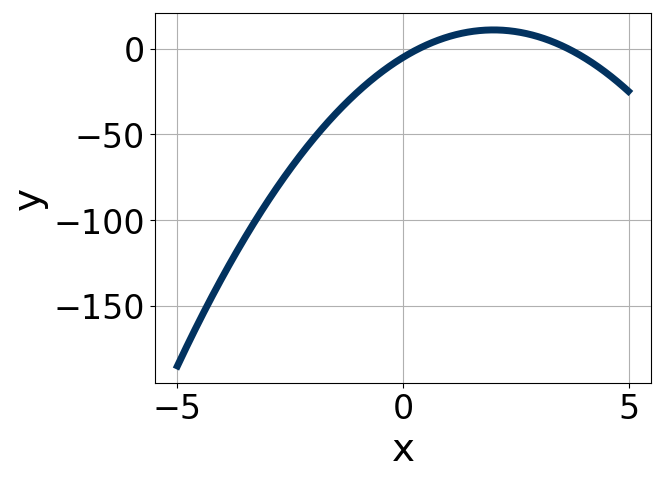
\includegraphics[width = 0.3\textwidth]{../Figures/quadraticEquationToGraphCC.png}\item 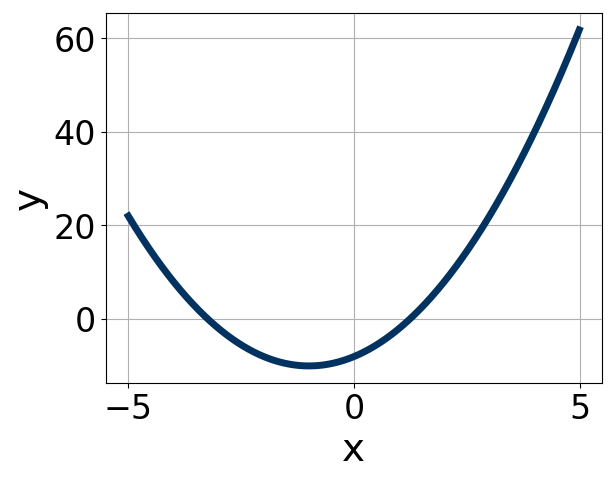
\includegraphics[width = 0.3\textwidth]{../Figures/quadraticEquationToGraphDC.png}\end{multicols}\item None of the above.
\end{enumerate} }
\end{enumerate}

\end{document}